\chapter{Экспериментальная часть}

В данном разделе описаны проведённые замеры и представлены их результаты. Также будут уточнены характеристики устройства, на котором проводились замеры.

\section{Технические характеристики}
Технические характеристики устройства, на котором выполнялось тестирование \cite{web_item5}:
\begin{itemize}
	\item операционная система macOS Monterey 12.4;
	\item 8 ГБ оперативной памяти;
	\item процессор Apple M2 (базовая частота~---~2400 МГц, но поддержка технологии Turbo Boost позволяет достигать частоты в 3500 МГц \cite{web_item10}).
\end{itemize}

\section{Измерение времени выполнения реализаций алгоритмов}
Замеры времени реализаций алгоритмов производилось при помощи импортируемой в $Go$ функции $clock\_gettime$ языка $C$ \cite{web_item12}. Эта функция при использовании макроса \\ $CLOCK\_PROCESS\_CPUTIME\_ID$ возвращает затраченное на работу процесса процессорное время в формате структуры $struct\ timespec$, в которой хранятся результаты замеров из двух частей~---~в секундах и наносекундах (см. листинг \ref{code:timespec}).

\begin{code}
\caption{Листинг структуры $struct\ timespec$}
\label{code:timespec}

\begin{minted}{c}
struct timespec {
	time_t   tv_sec;        /* seconds */
	long     tv_nsec;       /* nanoseconds */
};
\end{minted}
\end{code}

Количество повторений замера для одинаковых входных данных~---~100.

\newpage

Функция, возвращающая текущее процессорное время, приведена в листинге \ref{code:cpu}.

\begin{code}
\caption{Листинг функции, возвращающей текущее процессорное время}
\label{code:cpu}

\begin{minted}{c}
#include <pthread.h>
#include <time.h>
#include <stdio.h>

static long long getCPUNs(){
	struct timespec time;
	if (clock_gettime(CLOCK_PROCESS_CPUTIME_ID, &time)) {
		perror("can't measure time");
		return 0;
	}
	return time.tv_sec * 1000000000LL + time.tv_nsec;
}
\end{minted}
\end{code}

Функция единичного замера времени выполнения в наносекундах приведена в листинге \ref{code:measure}, где $alg.function$~---~объект типа функция (в данной реализации~---~функция, описывающая один из алгоритмов умножения матриц).

\begin{code}
\caption{Листинг функции единичного замера времени выполнения в наносекундах}
\label{code:measure}
\begin{minted}{c}
func RunBenchmark(m1, m2 matrix.Matrix, alg algorithm) int {
	t := 0

	start := C.getCPUNs()
	for i := 0; i < NumTests; i++ {
		alg.function(m1, m2)
	}
	end := C.getCPUNs()
	t = int(end-start) / NumTests

	return t
}

\end{minted}
\end{code}

Входные матрицы для проведения замеров заполняются случайными числами с помощью функции, реализация которой представлена в листинге \ref{code:gen}.
\begin{code}
\caption{Листинг примера функции для заполнения матрицы случайными числами в диапазоне от -500 до 500}
\label{code:gen}
\begin{minted}{go}
const (
	maxNum   = 1000
	interval = 500
)

func FillRandom(m Matrix) {
	for i := 0; i < m.M; i++ {
		for j := 0; j < m.N; j++ {
			m.Data[i][j] = rand.Intn(maxNum+1) - interval
		}
	}
}
\end{minted}
\end{code}

Результаты замеров времени выполнения (в нс) приведены в таблицах \ref{table:time1}~---~\ref{table:time2}. Оптимизации компилятора были отключены с помощью флага $-gcflags '-N -l'$. Для стандартного алгоритма умножения матриц невозможно выделить худший и лучший случай в зависимости от входных данных, поэтому понятия «худший» и «лучший случай», применительно к нижеописанным результатам замеров, относятся только к реализациям алгоритма Винограда. На рисунках \ref{img:graph1}~---~\ref{img:graph4} приведены графики, отображающие зависимость времени работы алгоритмов от размера матриц для лучшего и худшего случаев. Результаты замеров для реализаций алгоритмов Винограда вынесены на отдельный рисунок для каждого случая, так как разница в быстродействии невелика, что делает невозможность наглядно продемонстрировать её на большом диапазоне значений размерностей входных матриц. Матрицы заполнялись случайными числами.

\begin{table}[H]
  \caption{\label{table:time1} Результаты замеров времени для лучшего случая (чётная размерность) (нс)}
  \begin{center}
    \begin{tabular}{
    |S[table-format=4.0]
    |S[table-format=10.0]
    |S[table-format=10.0]
    |S[table-format=10.0]|
    }
      \hline
      {Размерность~матриц} & {Стандартный} & {Виноград} & {Опт.~Виноград} \\\hline
      2 & 180 & 330 & 280\\ \hline
      10 & 9220 & 3350 & 2790\\ \hline
      50 & 503320 & 277690 & 260000\\ \hline
      100 & 4261770 & 2178990 & 2159120\\ \hline
      200 & 36068900 & 19995980 & 19371750\\ \hline
      300 & 130022190 & 74695990 & 71111840\\ \hline
      500 & 599444020 & 334126470 & 327040510\\ \hline
    \end{tabular}
  \end{center}
\end{table}

\noindent
\begin{table}[h!]
  \centering
  \begin{tabular}{p{1\linewidth}}
    \centering
    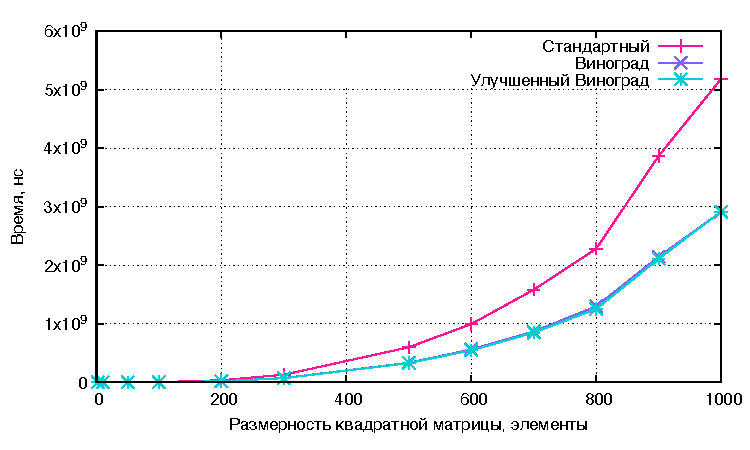
\includegraphics[width=0.85\linewidth]{../images/time_best.pdf}
    \captionof{figure}{Зависимость времени работы алгоритмов умножения матриц от размерности матриц (лучший случай)}
    \label{img:graph1}
  \end{tabular}
\end{table}

\noindent
\begin{table}[h!]
  \centering
  \begin{tabular}{p{1\linewidth}}
    \centering
    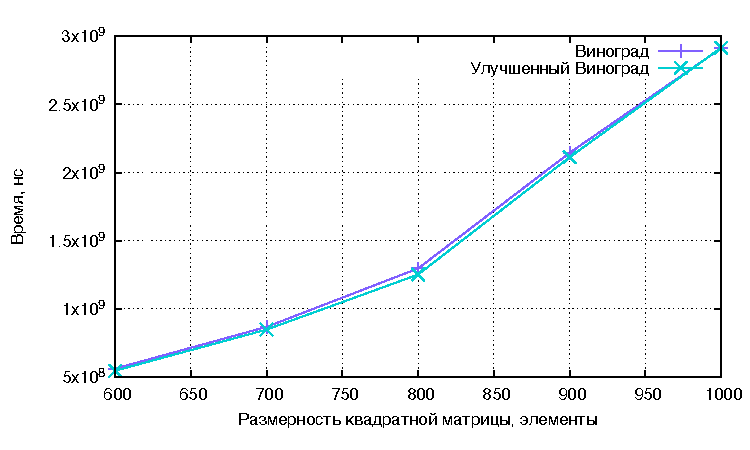
\includegraphics[width=0.85\linewidth]{../images/time_best_winograd.pdf}
    \captionof{figure}{Зависимость времени работы алгоритмов умножения матриц от размерности матриц (лучший случай, алгоритм Винограда)}
    \label{img:graph2}
  \end{tabular}
\end{table}

\newpage

\begin{table}[H]
  \caption{\label{table:time2} Результаты замеров времени для худшего случая (нечётная размерность) (нс)}
  \begin{center}
    \begin{tabular}{
    |S[table-format=4.0]
    |S[table-format=10.0]
    |S[table-format=10.0]
    |S[table-format=10.0]|
    }
      \hline
      {Размерность матриц} & {Стандартный} & {Виноград} & {Опт.~Виноград} \\ \hline
      2 & 330 & 430 & 333\\ \hline
      10 & 4940 & 3890 & 3590\\ \hline
      50 & 538720 & 290780 & 288490\\ \hline
      100 & 4401290 & 2264800 & 2223520\\ \hline
      200 & 36774650 & 20298640 & 19554690\\ \hline
      300 & 131696540 & 74210140 & 71339110\\ \hline
      500 & 604239010 & 335168220 & 328529920\\ \hline
    \end{tabular}
  \end{center}
\end{table}

\noindent
\begin{table}[h!]
  \centering
  \begin{tabular}{p{1\linewidth}}
    \centering
    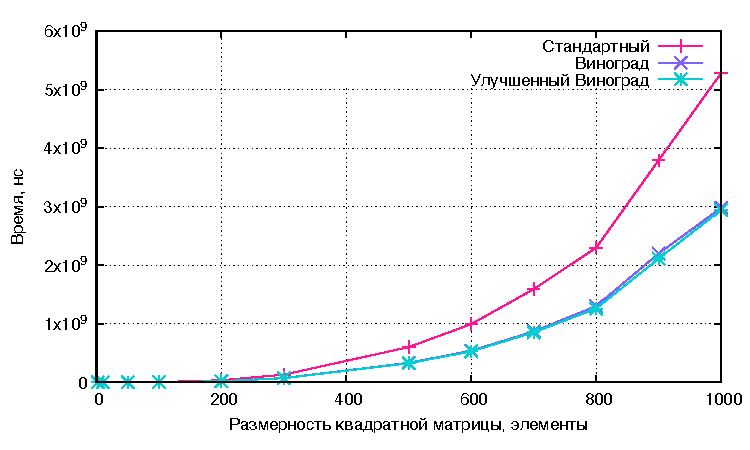
\includegraphics[width=0.8\linewidth]{../images/time_worst.pdf}
    \captionof{figure}{Зависимость времени работы алгоритмов умножения матриц от размерности матриц (худший случай)}
    \label{img:graph3}
  \end{tabular}
\end{table}

\noindent
\begin{table}[h!]
  \centering
  \begin{tabular}{p{1\linewidth}}
    \centering
    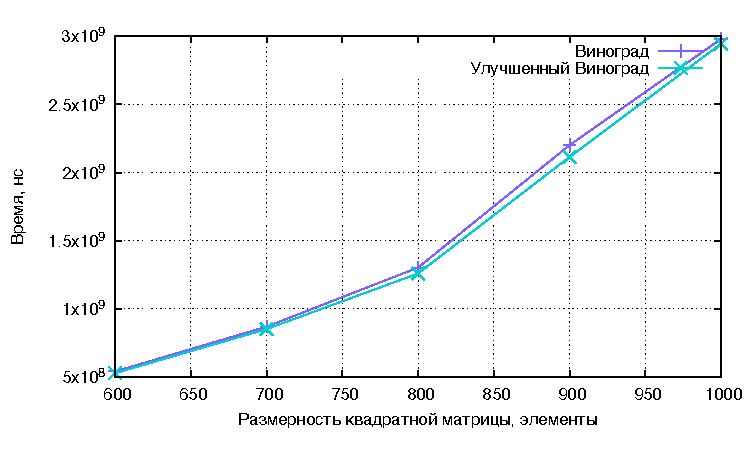
\includegraphics[width=0.95\linewidth]{../images/time_worst_winograd.pdf}
    \captionof{figure}{Зависимость времени работы алгоритмов умножения матриц от размерности матриц (худший случай, алгоритм Винограда)}
    \label{img:graph4}
  \end{tabular}
\end{table}

\section{Измерение объёма потребляемой памяти реализаций}
Измерение объёма потребляемой памяти производилось посредством создания собственного программного модуля memory, использующего функции пакета unsafe языка $Go$ \cite{web_item3}. Реализация основного функционала модуля, а также пример функции расчёта памяти, затрачиваемой на стандартный алгоритм умножения матриц, и пример использования указанных функций приведены в Приложении А.

Результаты замеров потребляемой памяти (в байтах) приведены в таблице \ref{table:mem}. На рисунке \ref{img:graph5} приведён график, отображающий зависимость потребляемой памяти от размерности матриц. Матрицы заполнялись случайными числами. Результаты замеров на графике представлены на диапазоне размерностей матриц до 100 из-за незначительности разницы в потреблении памяти, что не позволяет наглядно продемонстрировать её на большом диапазоне значений размерностей входных матриц.

\begin{table}[h]
  \caption{\label{table:mem} Результаты замеров потребляемой памяти (в байтах)}
  \begin{center}
    \begin{tabular}{
    |S[table-format=4.0]
    |S[table-format=10.0]
    |S[table-format=10.0]
    |S[table-format=10.0]|
    }
      \hline
      {Размерность матриц} & {Стандартный} & {Виноград} & {Опт.~Виноград} \\ \hline
      2 & 272 & 544 & 552\\ \hline
      10 & 1232 & 1632 & 1640\\ \hline
      50 & 21392 & 22432 & 22440\\ \hline
      100 & 82592 & 84432 & 84440\\ \hline
      200 & 324992 & 328432 & 328440\\ \hline
      300 & 727392 & 732432 & 732440\\ \hline
      500 & 2012192 & 2020432 & 2020440\\ \hline
    \end{tabular}
  \end{center}
\end{table}

\newpage

\noindent
\begin{figure}[t!]
	\centering
    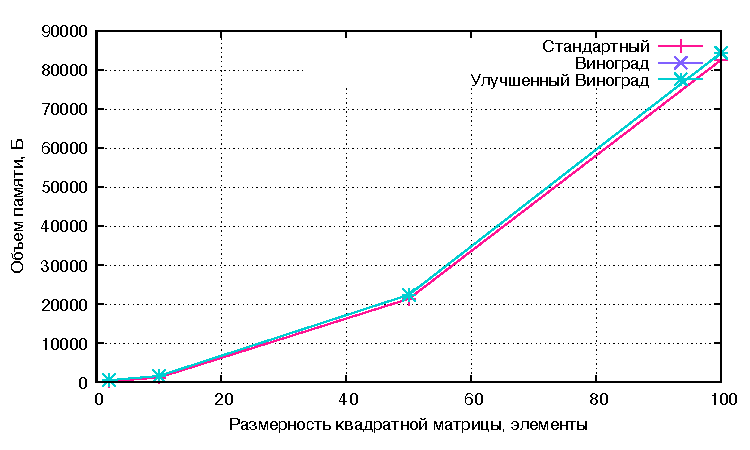
\includegraphics[width=0.95\linewidth]{../images/memory.pdf}
    \caption{Зависимость потребляемой памяти от размерности матриц при умножении}
    \label{img:graph5}
\end{figure}

\newpage